\subsection{Integratietesten}
Alle belangrijke interacties tussen de componenten zijn getest door middel van integratie testen.
Deze testen zijn ook gemaakt in xUnit een van de geïmplementeerde testen is te zien in figuur \ref{fig:IntergrationTest}.
In het voorbeeld is te zien dat er gebruik wordt gemaakt van het mocken van de repository.
Mocken is het gebruiken van een \qw{nep} implementatie van de gebruikte interface. 
Hierdoor is het mogelijk om aan te geven welke specifieke methode terugverwacht wordt.
% Hierdoor kan je aangeven wat je specifiek van een methode terugverwacht.
Omdat er gebruikgemaakt wordt van het repository pattern is het makkelijk om de database te mocken.
Verder is er een overzicht te zien van alle testen in figuur \ref{fig:OverviewUnitTests}.


\whitespace[2]
\begin{graphic}
	\captionsetup{type=figure}
	\caption{Geïmplementeerde integratie test}
	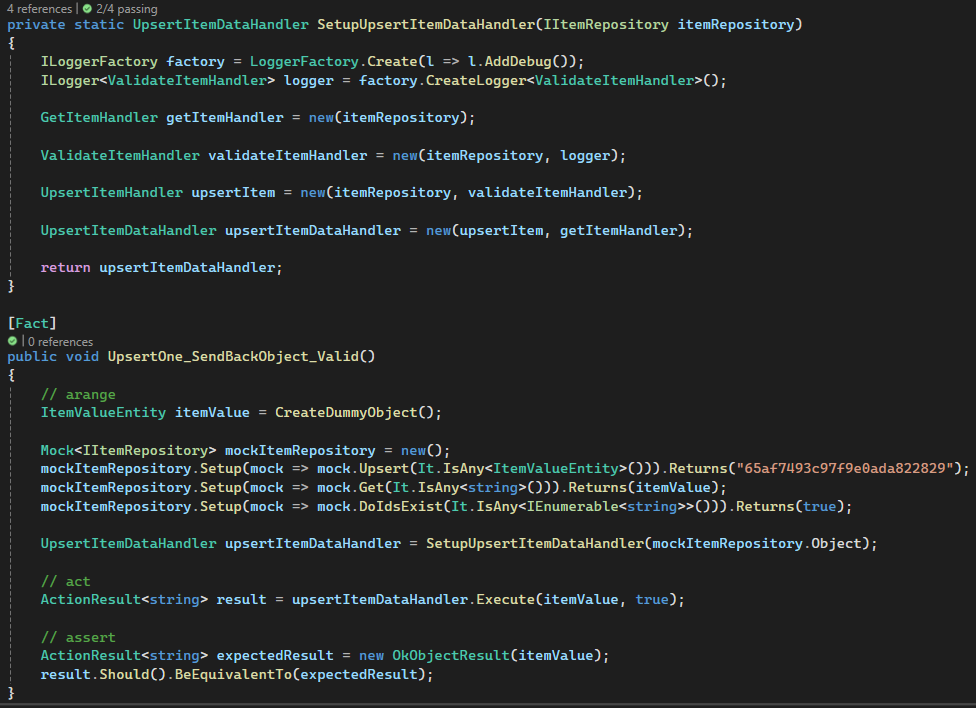
\includegraphics[scale=0.58]{IntergrationTestExample.png}
	\label{fig:IntergrationTest}
\end{graphic}

\whitespace[2]
\begin{graphic}
	\captionsetup{type=figure}
	\caption{Overzicht integratie en unittesten}
	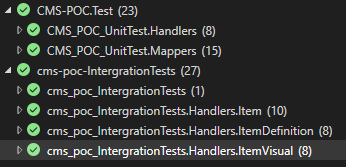
\includegraphics[scale=1]{OverzichtUnitTesten.png}
	\label{fig:OverviewUnitTests}
\end{graphic}
